\chapter{Appendix A: Scanning techniques comparison}
\pagenumbering{roman}
\label{appendix:appendix-a}

\section{Experiment Parameters}
\label{appendix:expirement-parameters}
%% \begin{figure}[ht]
%% \begin{tabular}{p{5cm}p{5cm}p{5cm}}
\begin{itemize}
\item Operating system:
    \begin{itemize}
    \item Windows 10.0.19042.1889
    \item Ubuntu 22.04 (LTS)
    \end{itemize}
\item Browser:
    \begin{itemize}
    \item Chrome 114.0.5735.91
    \item FireFox 115.0.2
    \end{itemize}
\item Scanning technique:
    \begin{itemize}
    \item Fetch
    \item XHR
    \item WebSocket
    \end{itemize}
\item Socket settings:
    \begin{itemize}
    \item Parallel sockets: 1, 5, 10, 20, 30, 40, 50, 60, 70, 100, 150, 200, 250
    \item Socket timeout settings: 100ms, 150ms, 200ms, 250ms, 300ms, 400ms 
    \end{itemize}
\item Artificially opened ports:
    \begin{itemize}
    \item N HTTP servers: 10, 33, 50, 100
    \end{itemize}
\end{itemize}

\clearpage
\section{Socket timeout comparison}

\begin{table}[htbp]
\footnotesize
\centering
\begin{adjustwidth}{-1.0cm}{}
\begin{tabular}{p{6.3cm}p{1.5cm}p{3cm}p{2cm}p{2cm}}
    \toprule
    Base Image & Browser & Socket timeout (ms) & Scanning Technique & Detected ports \\
     \midrule
    mcr.microsoft.com/windows:20H2-amd64 & Chrome & 100 & Fetch & 76 \\
    mcr.microsoft.com/windows:20H2-amd64 & Chrome & 150, 200, 250, 300, 350, 400 & Fetch & 100 \\
    mcr.microsoft.com/windows:20H2-amd64 & Chrome & 100, 150, 200, 250, 300, 350, 400, 1000 & WebSocket, XHR & 0 \\
    \midrule
    mcr.microsoft.com/windows:20H2-amd64 & Firefox & 100 & Fetch & 21 \\
    mcr.microsoft.com/windows:20H2-amd64 & Firefox & 150, 200, 250, 300, 350, 400 & Fetch & 100 \\
    mcr.microsoft.com/windows:20H2-amd64 & Firefox & 100, 150, 200, 250, 300, 350, 400, 1000 & WebSocket, XHR & 0 \\
    \midrule
    library/ubuntu:22.04 & Chrome & 100, 150, 200, 250, 300, 350, 400 & Fetch & 100 \\
    library/ubuntu:22.04 & Chrome & 100, 150, 200, 250, 300, 350, 400 & WebSocket, XHR & 0 \\
    \midrule
    library/ubuntu:22.04 & Firefox & 100, 150, 200, 250, 300, 350, 400 & Fetch & 100 \\
    library/ubuntu:22.04 & Firefox & 100, 150, 200, 250, 300, 350, 400 & WebSocket, XHR & 0 \\
     \bottomrule
\end{tabular}
\end{adjustwidth}{}
\caption{Number of ports detected based on socket timeout setting (100 open ports) -- Scans were rerun 5 times to verify the accuracy of the results.}
\label{tab:socket-timeout-comparison}
\end{table}
\clearpage


\section{Scanning technique efficacy comparison}

\begin{table}[htbp]
\footnotesize
\centering
\begin{adjustwidth}{-1.0cm}{}
\begin{tabular}{p{6.3cm}p{1.5cm}p{1.7cm}p{1cm}p{1.3cm}p{3cm}}
    \toprule
    Base Image & Browser & Scanning Technique & Open Ports & Ports Detected & Scan Duration (ms) \\
    \midrule
    mcr.microsoft.com/windows:20H2-amd64 & Chrome & Fetch & 10 & 10 & 1282.6 \\
    mcr.microsoft.com/windows:20H2-amd64 & Chrome & Fetch & 33 & 33 & 1313.5 \\
    mcr.microsoft.com/windows:20H2-amd64 & Chrome & Fetch & 50 & 50 & 13153.8 \\
    mcr.microsoft.com/windows:20H2-amd64 & Chrome & Fetch & 100 & 100 & 1177.4 \\
    \midrule
    mcr.microsoft.com/windows:20H2-amd64 & Chrome & WebSocket & 10 & 0 & 1463.5 \\
    mcr.microsoft.com/windows:20H2-amd64 & Chrome & WebSocket & 33 & 0 & 1454.0 \\
    mcr.microsoft.com/windows:20H2-amd64 & Chrome & WebSocket & 50 & 0 & 1464.3 \\
    mcr.microsoft.com/windows:20H2-amd64 & Chrome & WebSocket & 100 & 0 & 1457.1 \\
    \midrule
    mcr.microsoft.com/windows:20H2-amd64 & Chrome & XHR & 10 & 0 & 1277.4 \\
    mcr.microsoft.com/windows:20H2-amd64 & Chrome & XHR & 33 & 0 & 1303.3 \\
    mcr.microsoft.com/windows:20H2-amd64 & Chrome & XHR & 50 & 0 & 1313.5 \\
    mcr.microsoft.com/windows:20H2-amd64 & Chrome & XHR & 100 & 0 & 1097.2 \\
    \midrule
    library/ubuntu:22.04 & Chrome & Fetch & 10 & 10 & 104.5 \\
    library/ubuntu:22.04 & Chrome & Fetch & 33 & 33 & 133.4 \\
    library/ubuntu:22.04 & Chrome & Fetch & 50 & 50 & 160.9 \\
    library/ubuntu:22.04 & Chrome & Fetch & 100 & 100 & 209.4 \\
    \midrule
    library/ubuntu:22.04 & Chrome & WebSocket & 10 & 0 & 1217.6 \\
    library/ubuntu:22.04 & Chrome & WebSocket & 33 & 0 & 1216.5 \\
    library/ubuntu:22.04 & Chrome & WebSocket & 50 & 0 & 1260.0 \\
    library/ubuntu:22.04 & Chrome & WebSocket & 100 & 0 & 1216.6 \\
    \midrule
    library/ubuntu:22.04 & Chrome & XHR & 10 & 0 & 98.3 \\
    library/ubuntu:22.04 & Chrome & XHR & 33 & 0 & 135.3 \\
    library/ubuntu:22.04 & Chrome & XHR & 50 & 0 & 154.2 \\
    library/ubuntu:22.04 & Chrome & XHR & 100 & 0 & 231.9 \\

    \midrule
    mcr.microsoft.com/windows:20H2-amd64 & Firefox & Fetch & 10 & 10 & 2553 \\
    mcr.microsoft.com/windows:20H2-amd64 & Firefox & Fetch & 33 & 33 & 2561 \\
    mcr.microsoft.com/windows:20H2-amd64 & Firefox & Fetch & 50 & 50 & 2552 \\
    mcr.microsoft.com/windows:20H2-amd64 & Firefox & Fetch & 100 & 100 & 2386 \\
    \midrule
    mcr.microsoft.com/windows:20H2-amd64 & Firefox & WebSocket & 10 & 0 & 2627 \\
    mcr.microsoft.com/windows:20H2-amd64 & Firefox & WebSocket & 33 & 0 & 2629 \\
    mcr.microsoft.com/windows:20H2-amd64 & Firefox & WebSocket & 50 & 0 & 2511 \\
    mcr.microsoft.com/windows:20H2-amd64 & Firefox & WebSocket & 100 & 0 & 2284 \\
    \midrule
    mcr.microsoft.com/windows:20H2-amd64 & Firefox & XHR & 10 & 0 & 2536 \\
    mcr.microsoft.com/windows:20H2-amd64 & Firefox & XHR & 33 & 0 & 2569 \\
    mcr.microsoft.com/windows:20H2-amd64 & Firefox & XHR & 50 & 0 & 2592 \\
    mcr.microsoft.com/windows:20H2-amd64 & Firefox & XHR & 100 & 0 & 2308 \\
    \midrule
    library/ubuntu:22.04 & Firefox & Fetch & 10 & 10 & 286 \\
    library/ubuntu:22.04 & Firefox & Fetch & 33 & 33 & 307 \\
    library/ubuntu:22.04 & Firefox & Fetch & 50 & 50 & 282 \\
    library/ubuntu:22.04 & Firefox & Fetch & 100 & 100 & 299 \\
    \midrule
    library/ubuntu:22.04 & Firefox & WebSocket & 10 & 0 & 268 \\
    library/ubuntu:22.04 & Firefox & WebSocket & 33 & 0 & 276 \\
    library/ubuntu:22.04 & Firefox & WebSocket & 50 & 0 & 290 \\
    library/ubuntu:22.04 & Firefox & WebSocket & 100 & 0 & 270 \\
    \midrule
    library/ubuntu:22.04 & Firefox & XHR & 10 & 0 & 254 \\
    library/ubuntu:22.04 & Firefox & XHR & 33 & 0 & 297 \\
    library/ubuntu:22.04 & Firefox & XHR & 50 & 0 & 287 \\
    library/ubuntu:22.04 & Firefox & XHR & 100 & 0 & 307 \\
     \bottomrule
\end{tabular}
\end{adjustwidth}{}
\caption{Scanning techniques comparison detecting HTTP ports. 50 parallel connections, 200ms socket timeout on Chrome, 400ms timeout on Firefox, 300 ports scanned.}

\label{tab:scan-technique-comparison}
\end{table}

\clearpage

Note that the results in Table~\ref{tab:scan-technique-comparison} do not mark ports as detected if they can be detected through post-scan analysis. The next section showcases the ability to detect open ports through post-scan analysis.


\section{Post-scan analysis efficacy comparison}
\label{appendix:scan-duration-comparison}
Scanning technique comparison through post-scan analysis. Comparing response times between open and closed ports.

\begin{figure}[ht]
\centering
\begin{minipage}{.45\textwidth}
  \centering
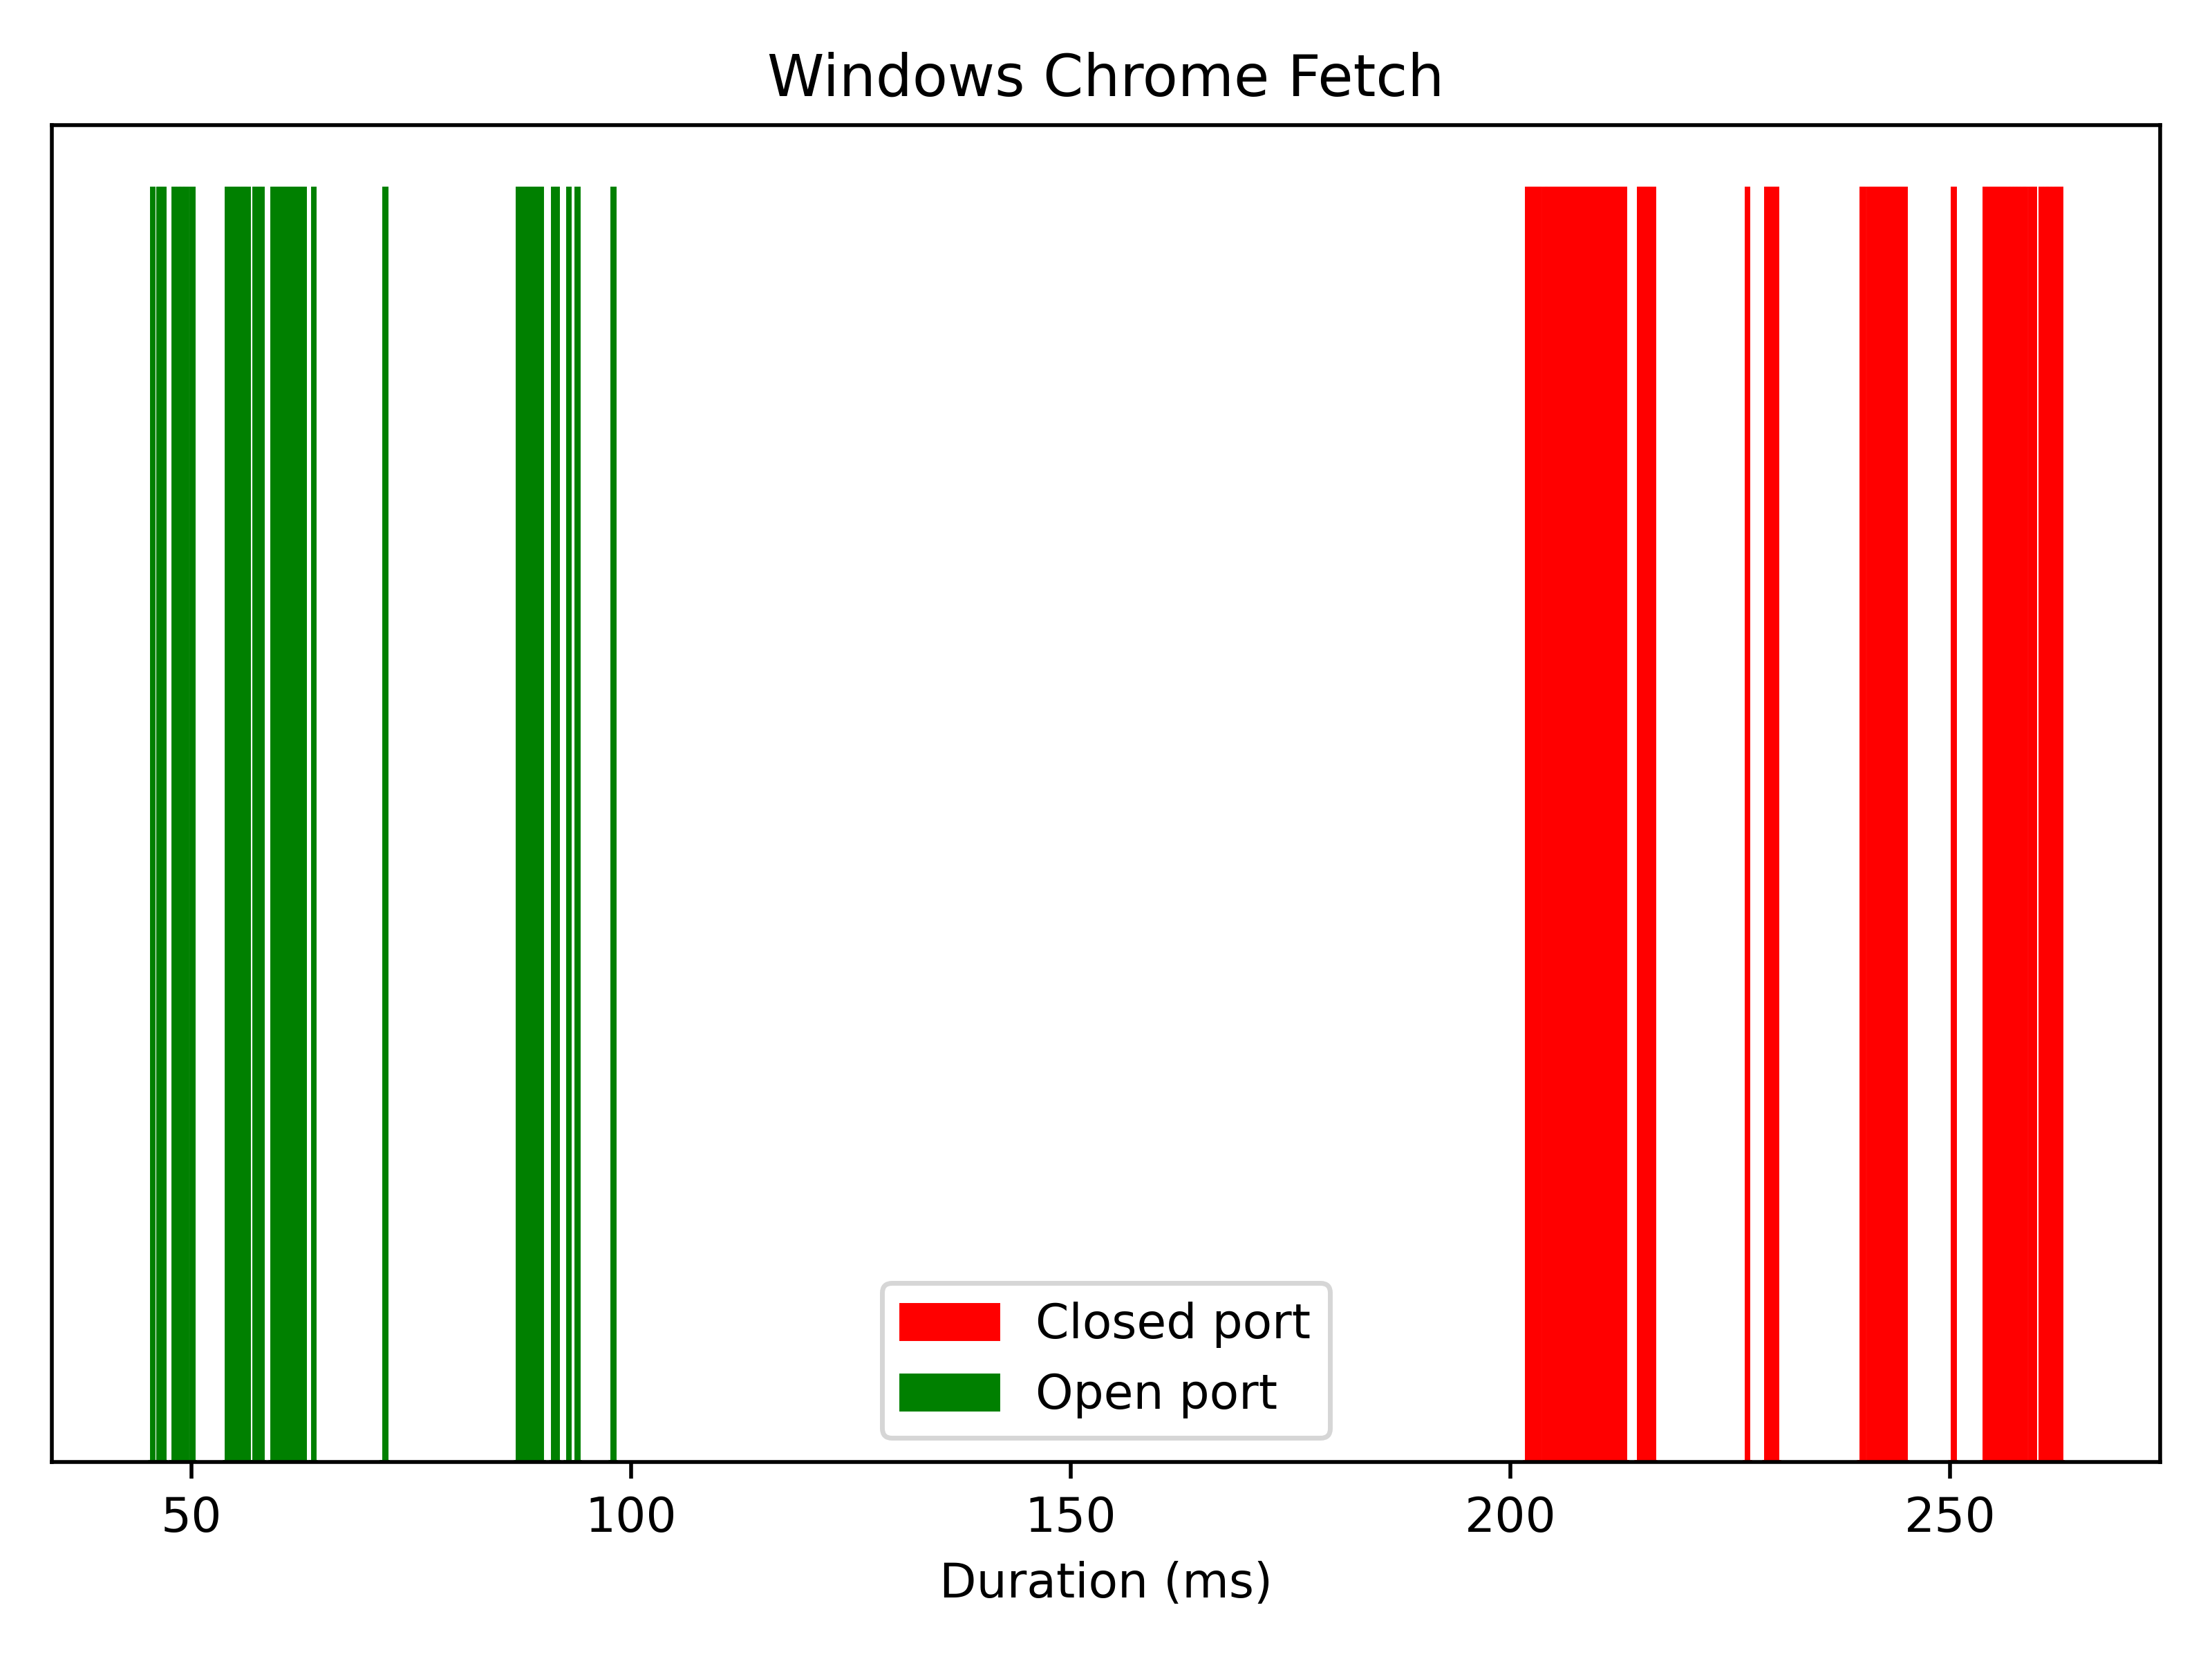
\includegraphics[width=8cm, height=4cm, keepaspectratio]{port_scanning_techniques/img/windows_chrome_efficacy_fetch.png}
    \caption{Windows/Chrome Fetch API scan duration open vs closed ports}
    \label{fig:win-chrome-fetch}
\end{minipage}
\hspace{0.5cm} % Adjust the horizontal space between the two figures
\begin{minipage}{.45\textwidth}
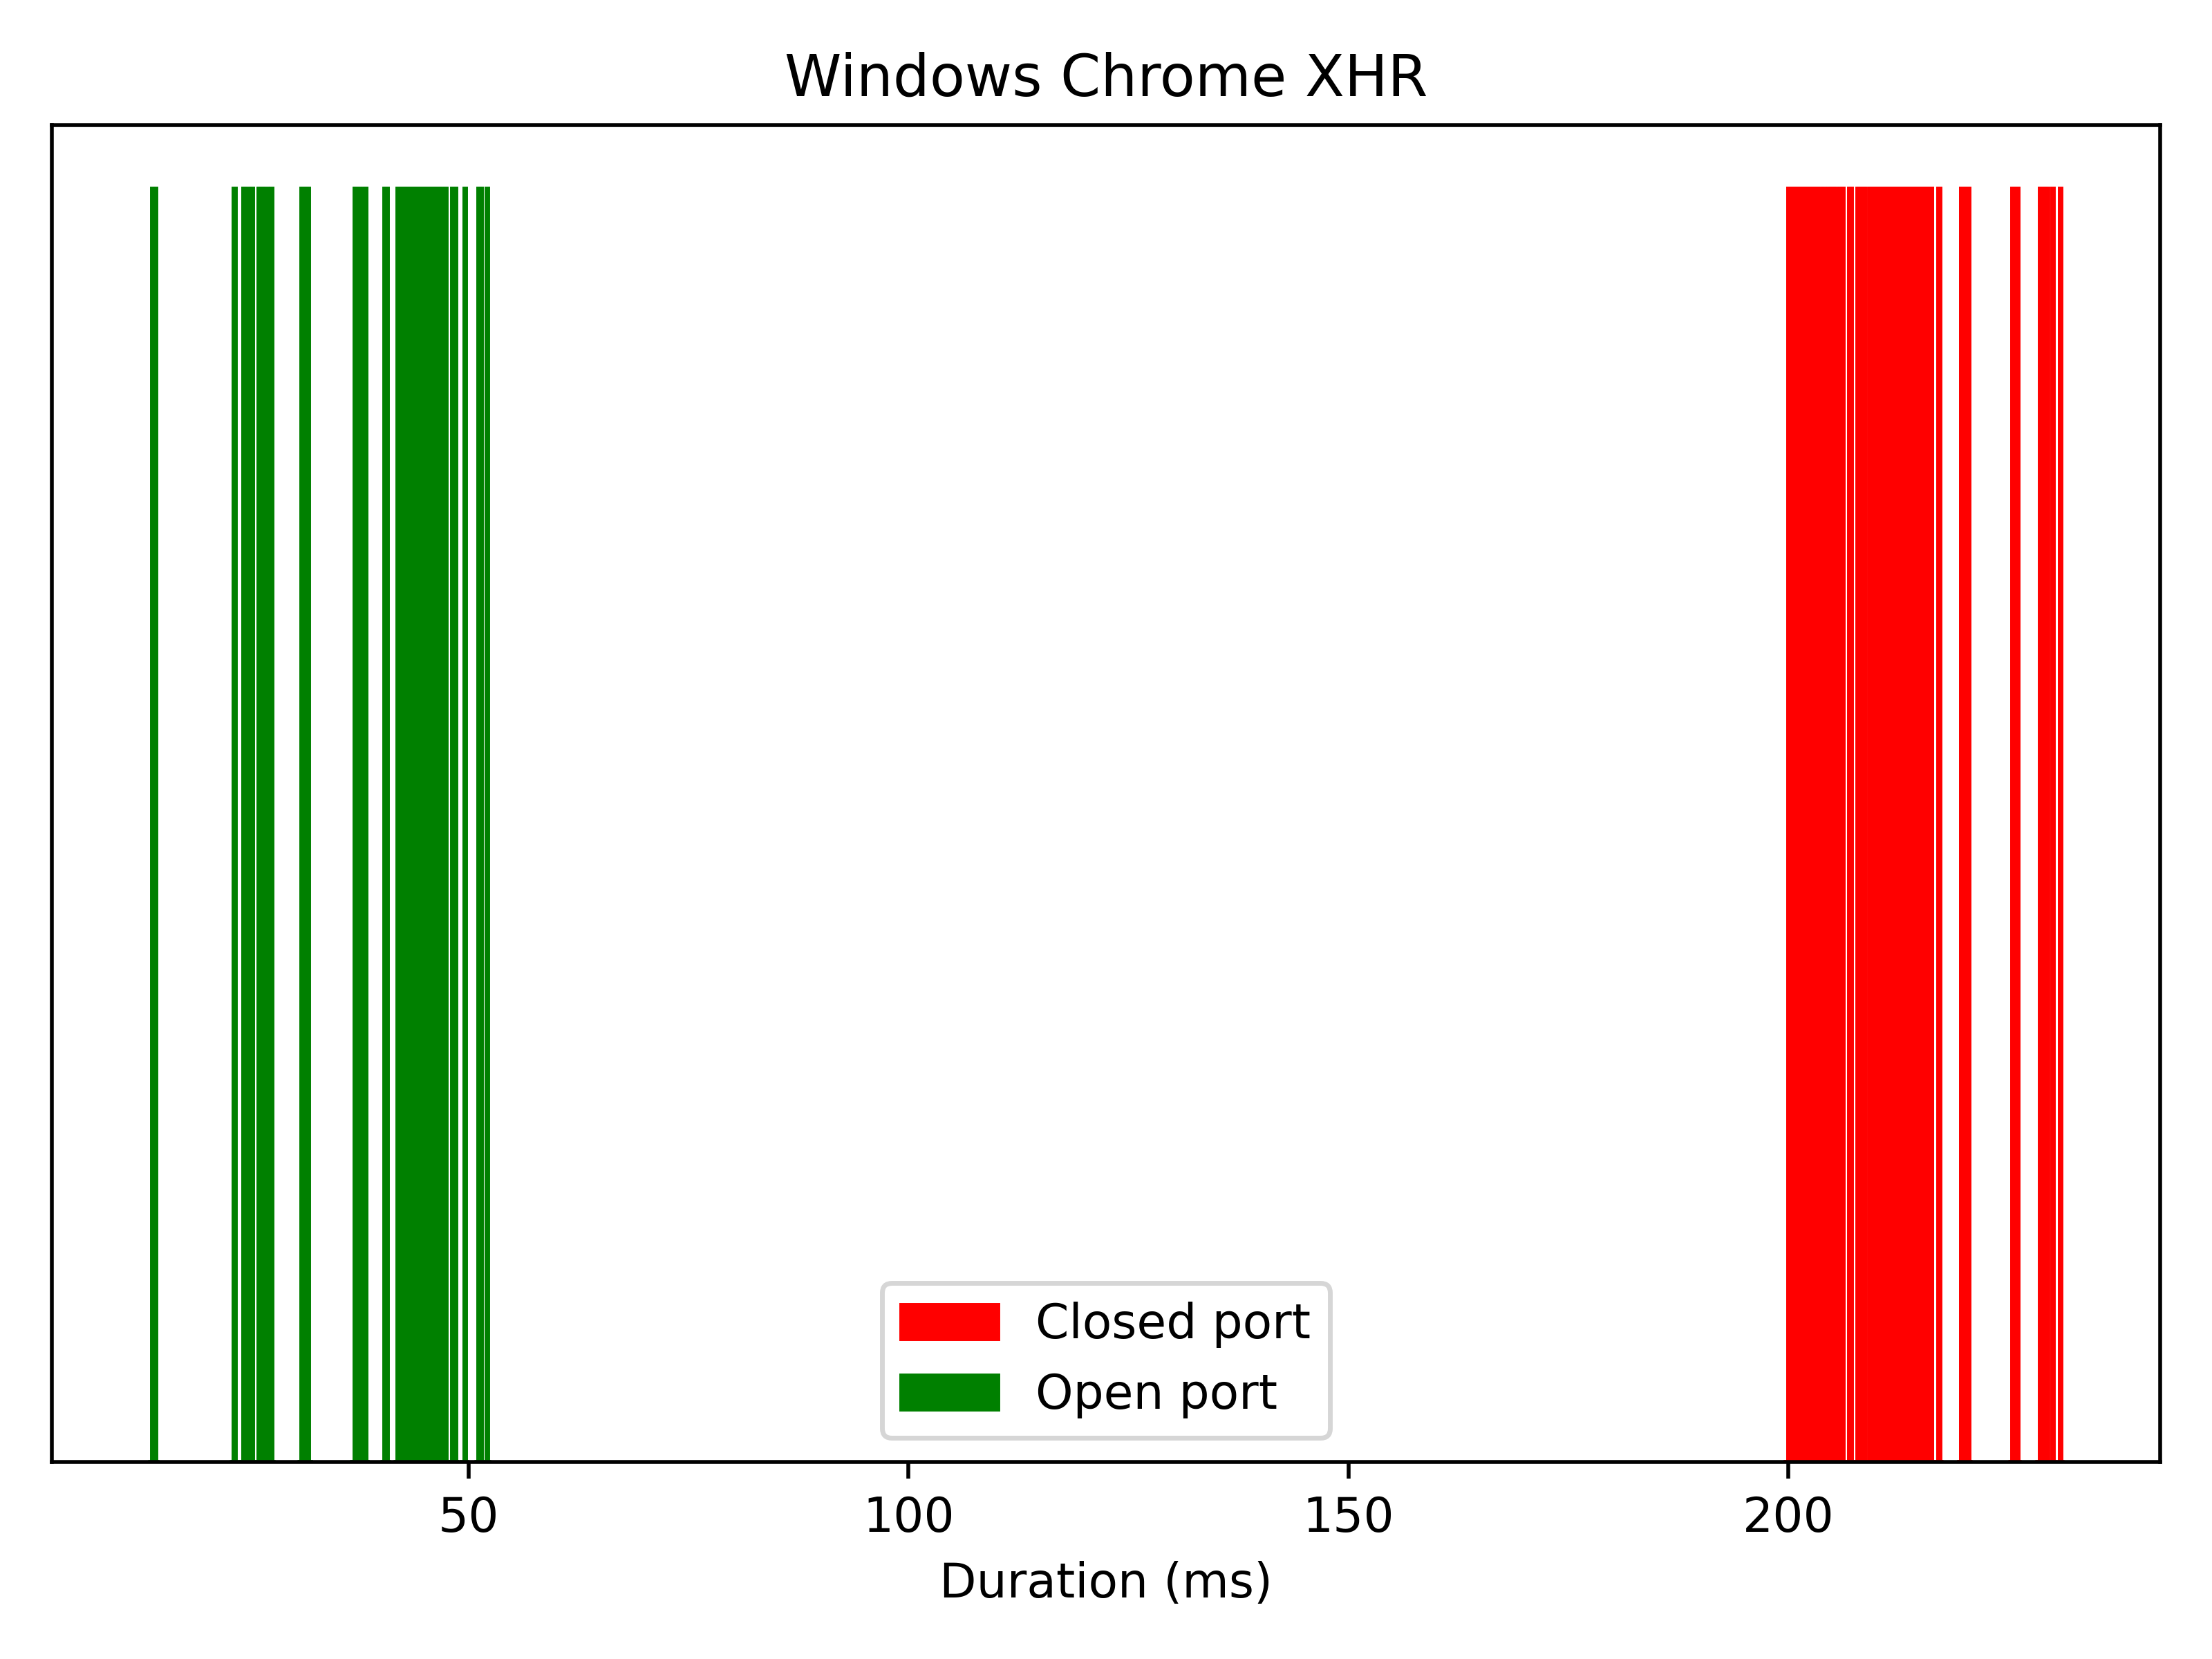
\includegraphics[width=8cm, height=4cm, keepaspectratio]{port_scanning_techniques/img/windows_chrome_efficacy_xhr.png}
    \caption{Windows/Chrome XHR API scan duration open vs closed ports}
    \label{fig:appendix-win-chrome-xhr}
\end{minipage}
\end{figure}

\begin{figure}[ht]
\centering
\begin{minipage}{.45\textwidth}
  \centering
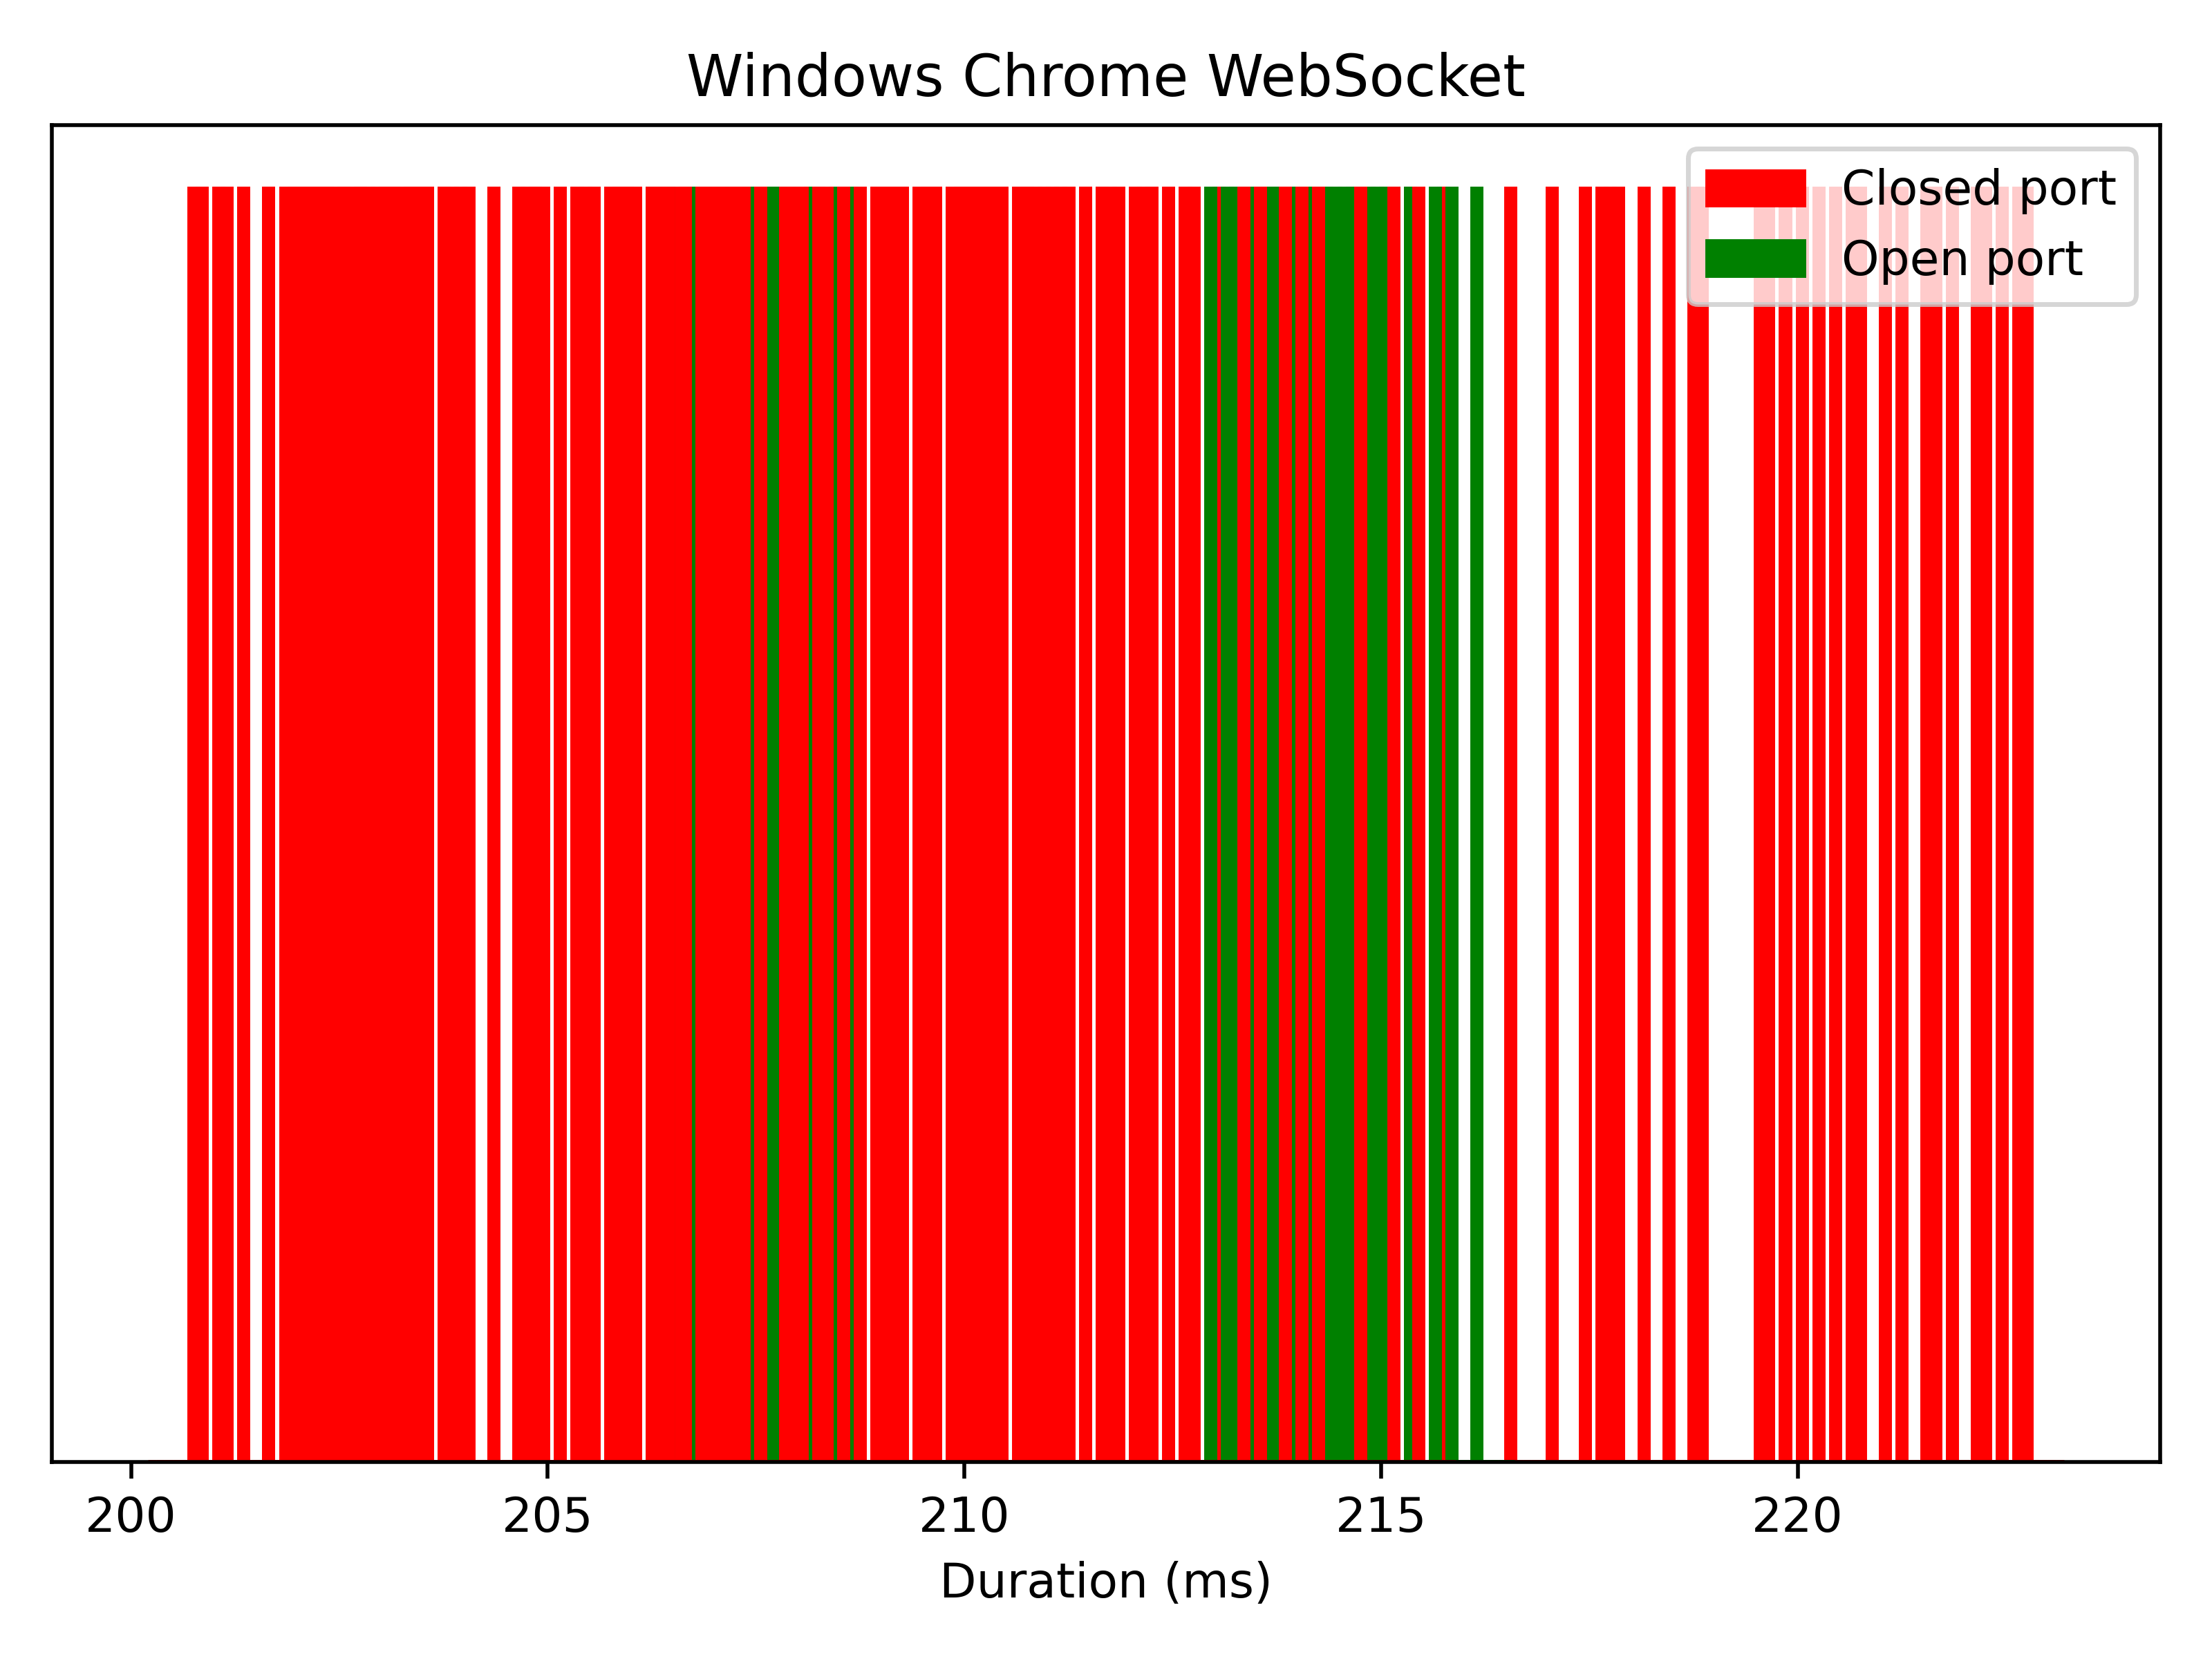
\includegraphics[width=8cm, height=4cm, keepaspectratio]{port_scanning_techniques/img/windows_chrome_efficacy_websocket.png}
    \caption{Windows/Chrome WebSocket API scan duration open vs closed ports}
    \label{fig:appendix-win-chrome-websocket}
\end{minipage}
\hspace{0.5cm} % Adjust the horizontal space between the two figures
\begin{minipage}{.45\textwidth}
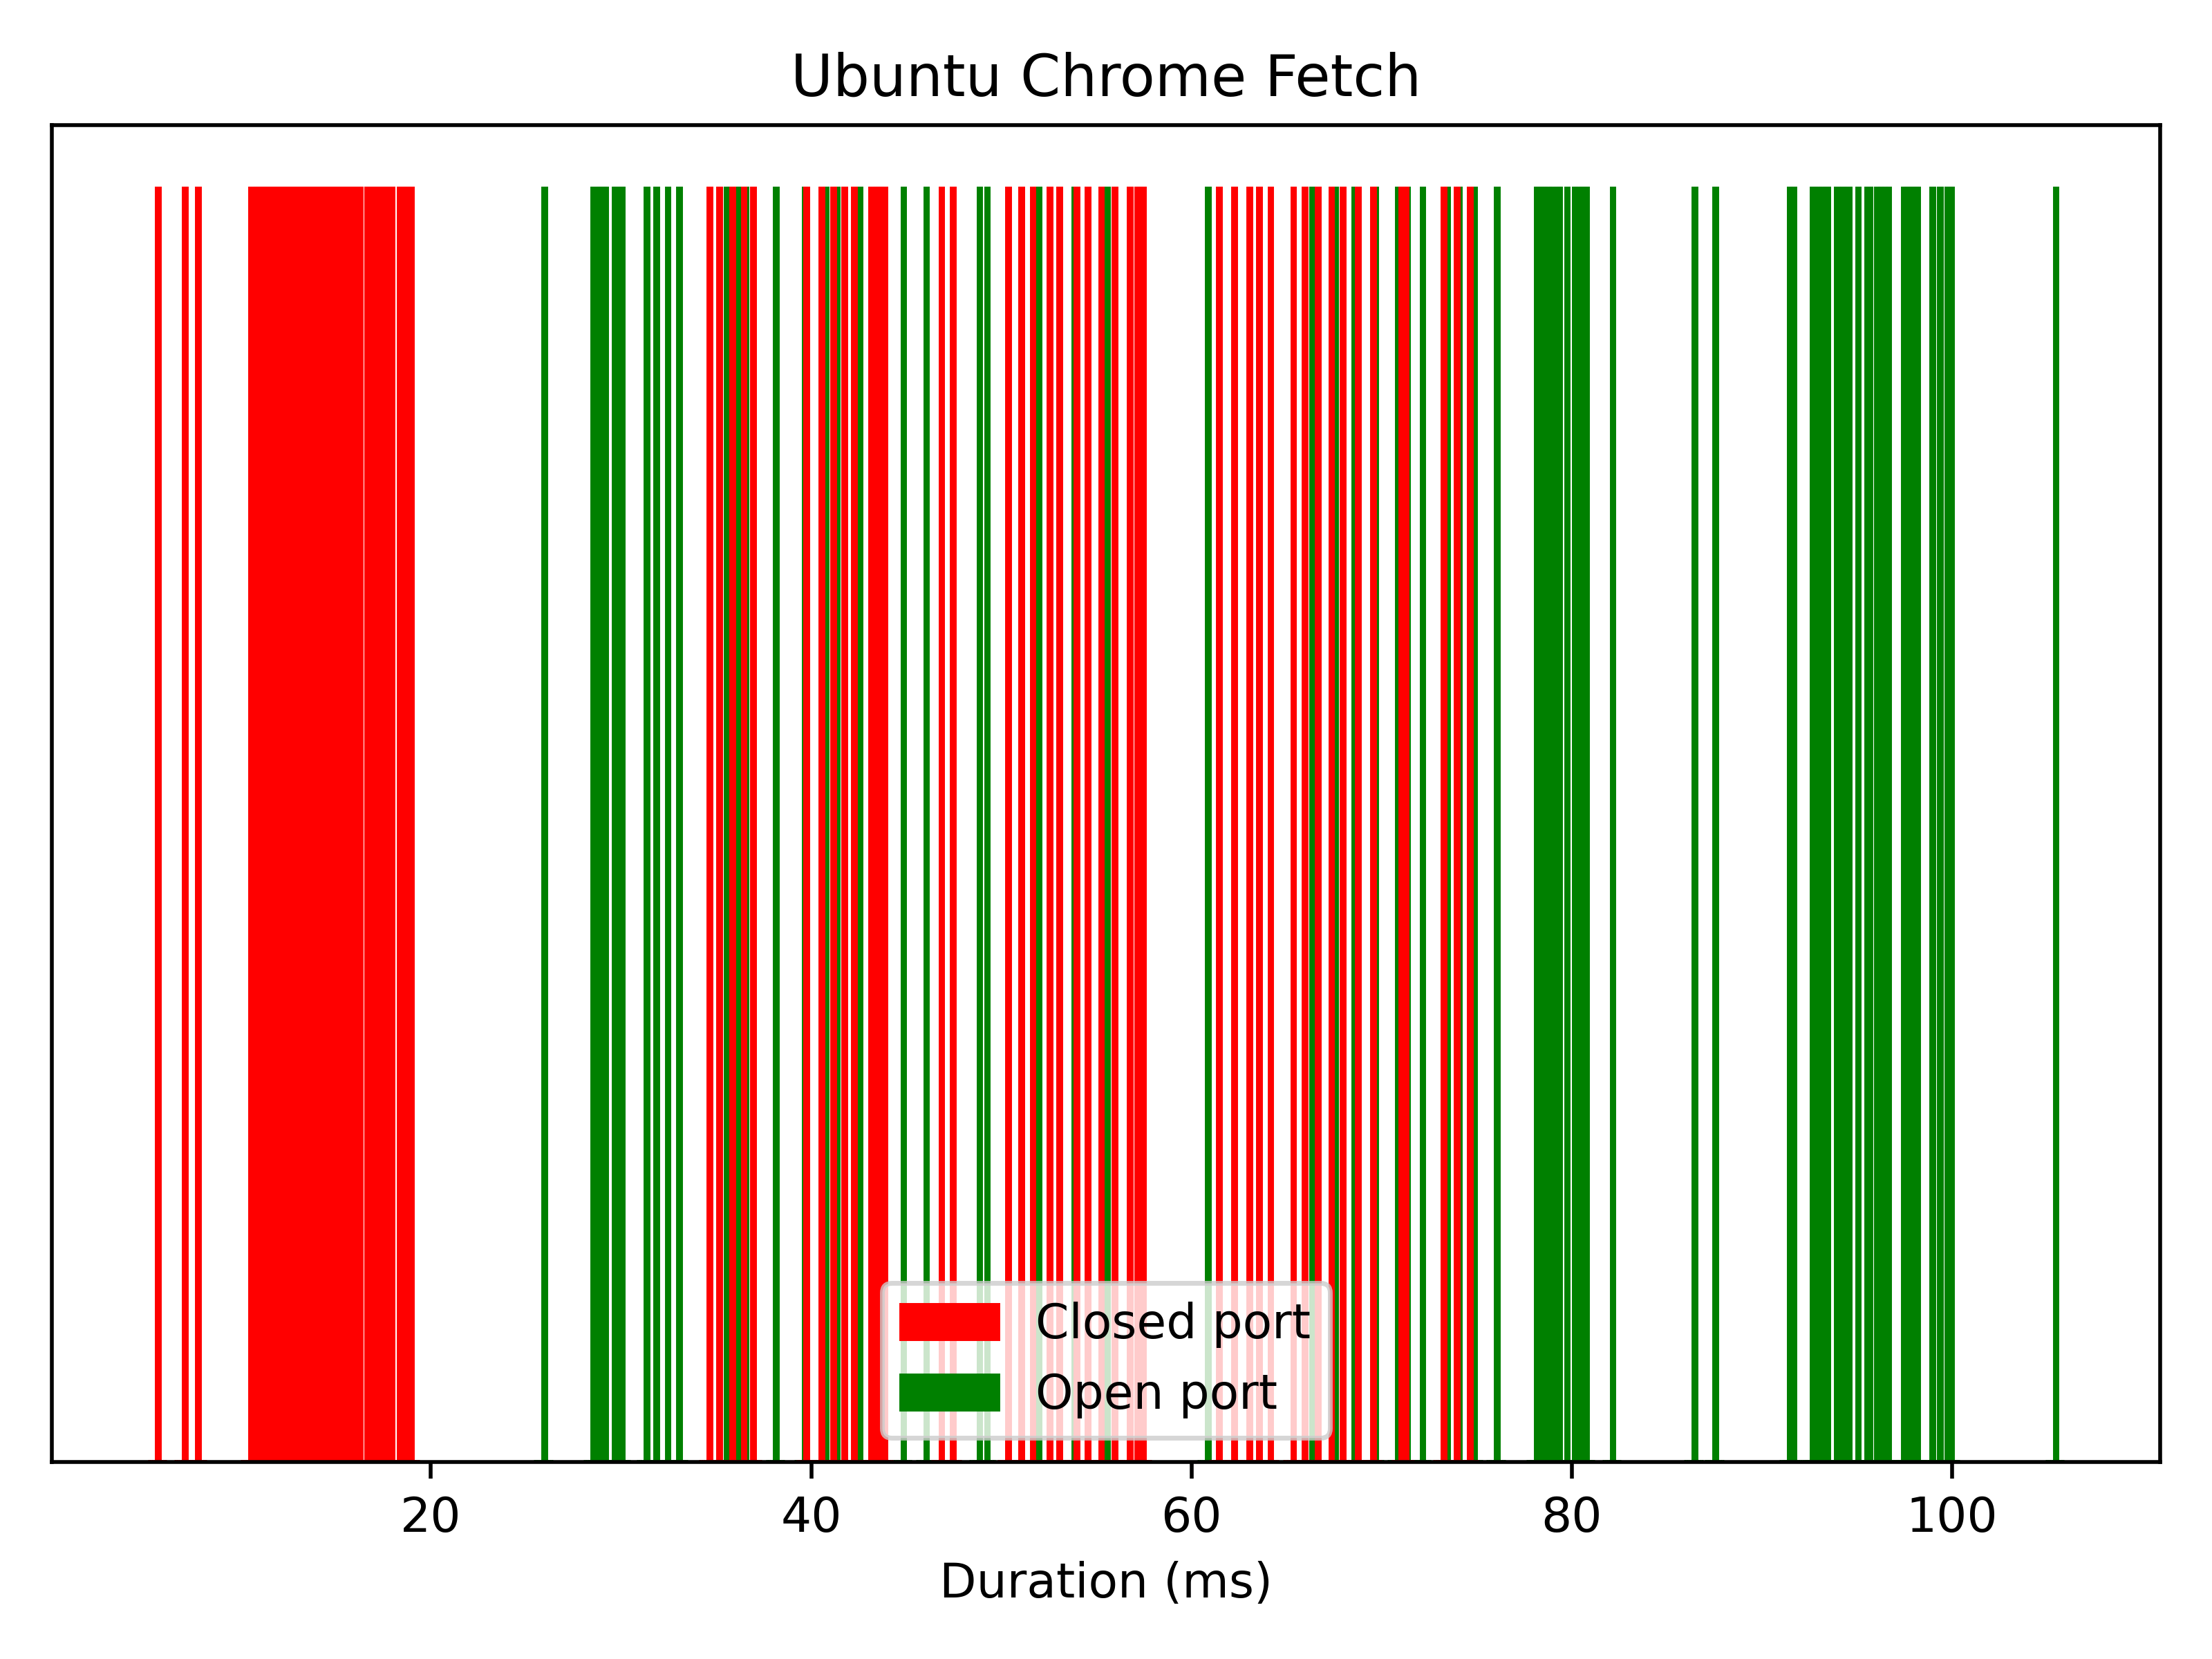
\includegraphics[width=8cm, height=4cm, keepaspectratio]{port_scanning_techniques/img/ubuntu_chrome_efficacy_fetch.png}
    \caption{Ubuntu/Chrome Fetch API scan duration open vs closed ports}
    \label{fig:ubuntu-chrome-fetch}
\end{minipage}
\end{figure}

\begin{figure}[ht]
\centering
\begin{minipage}{.45\textwidth}
  \centering
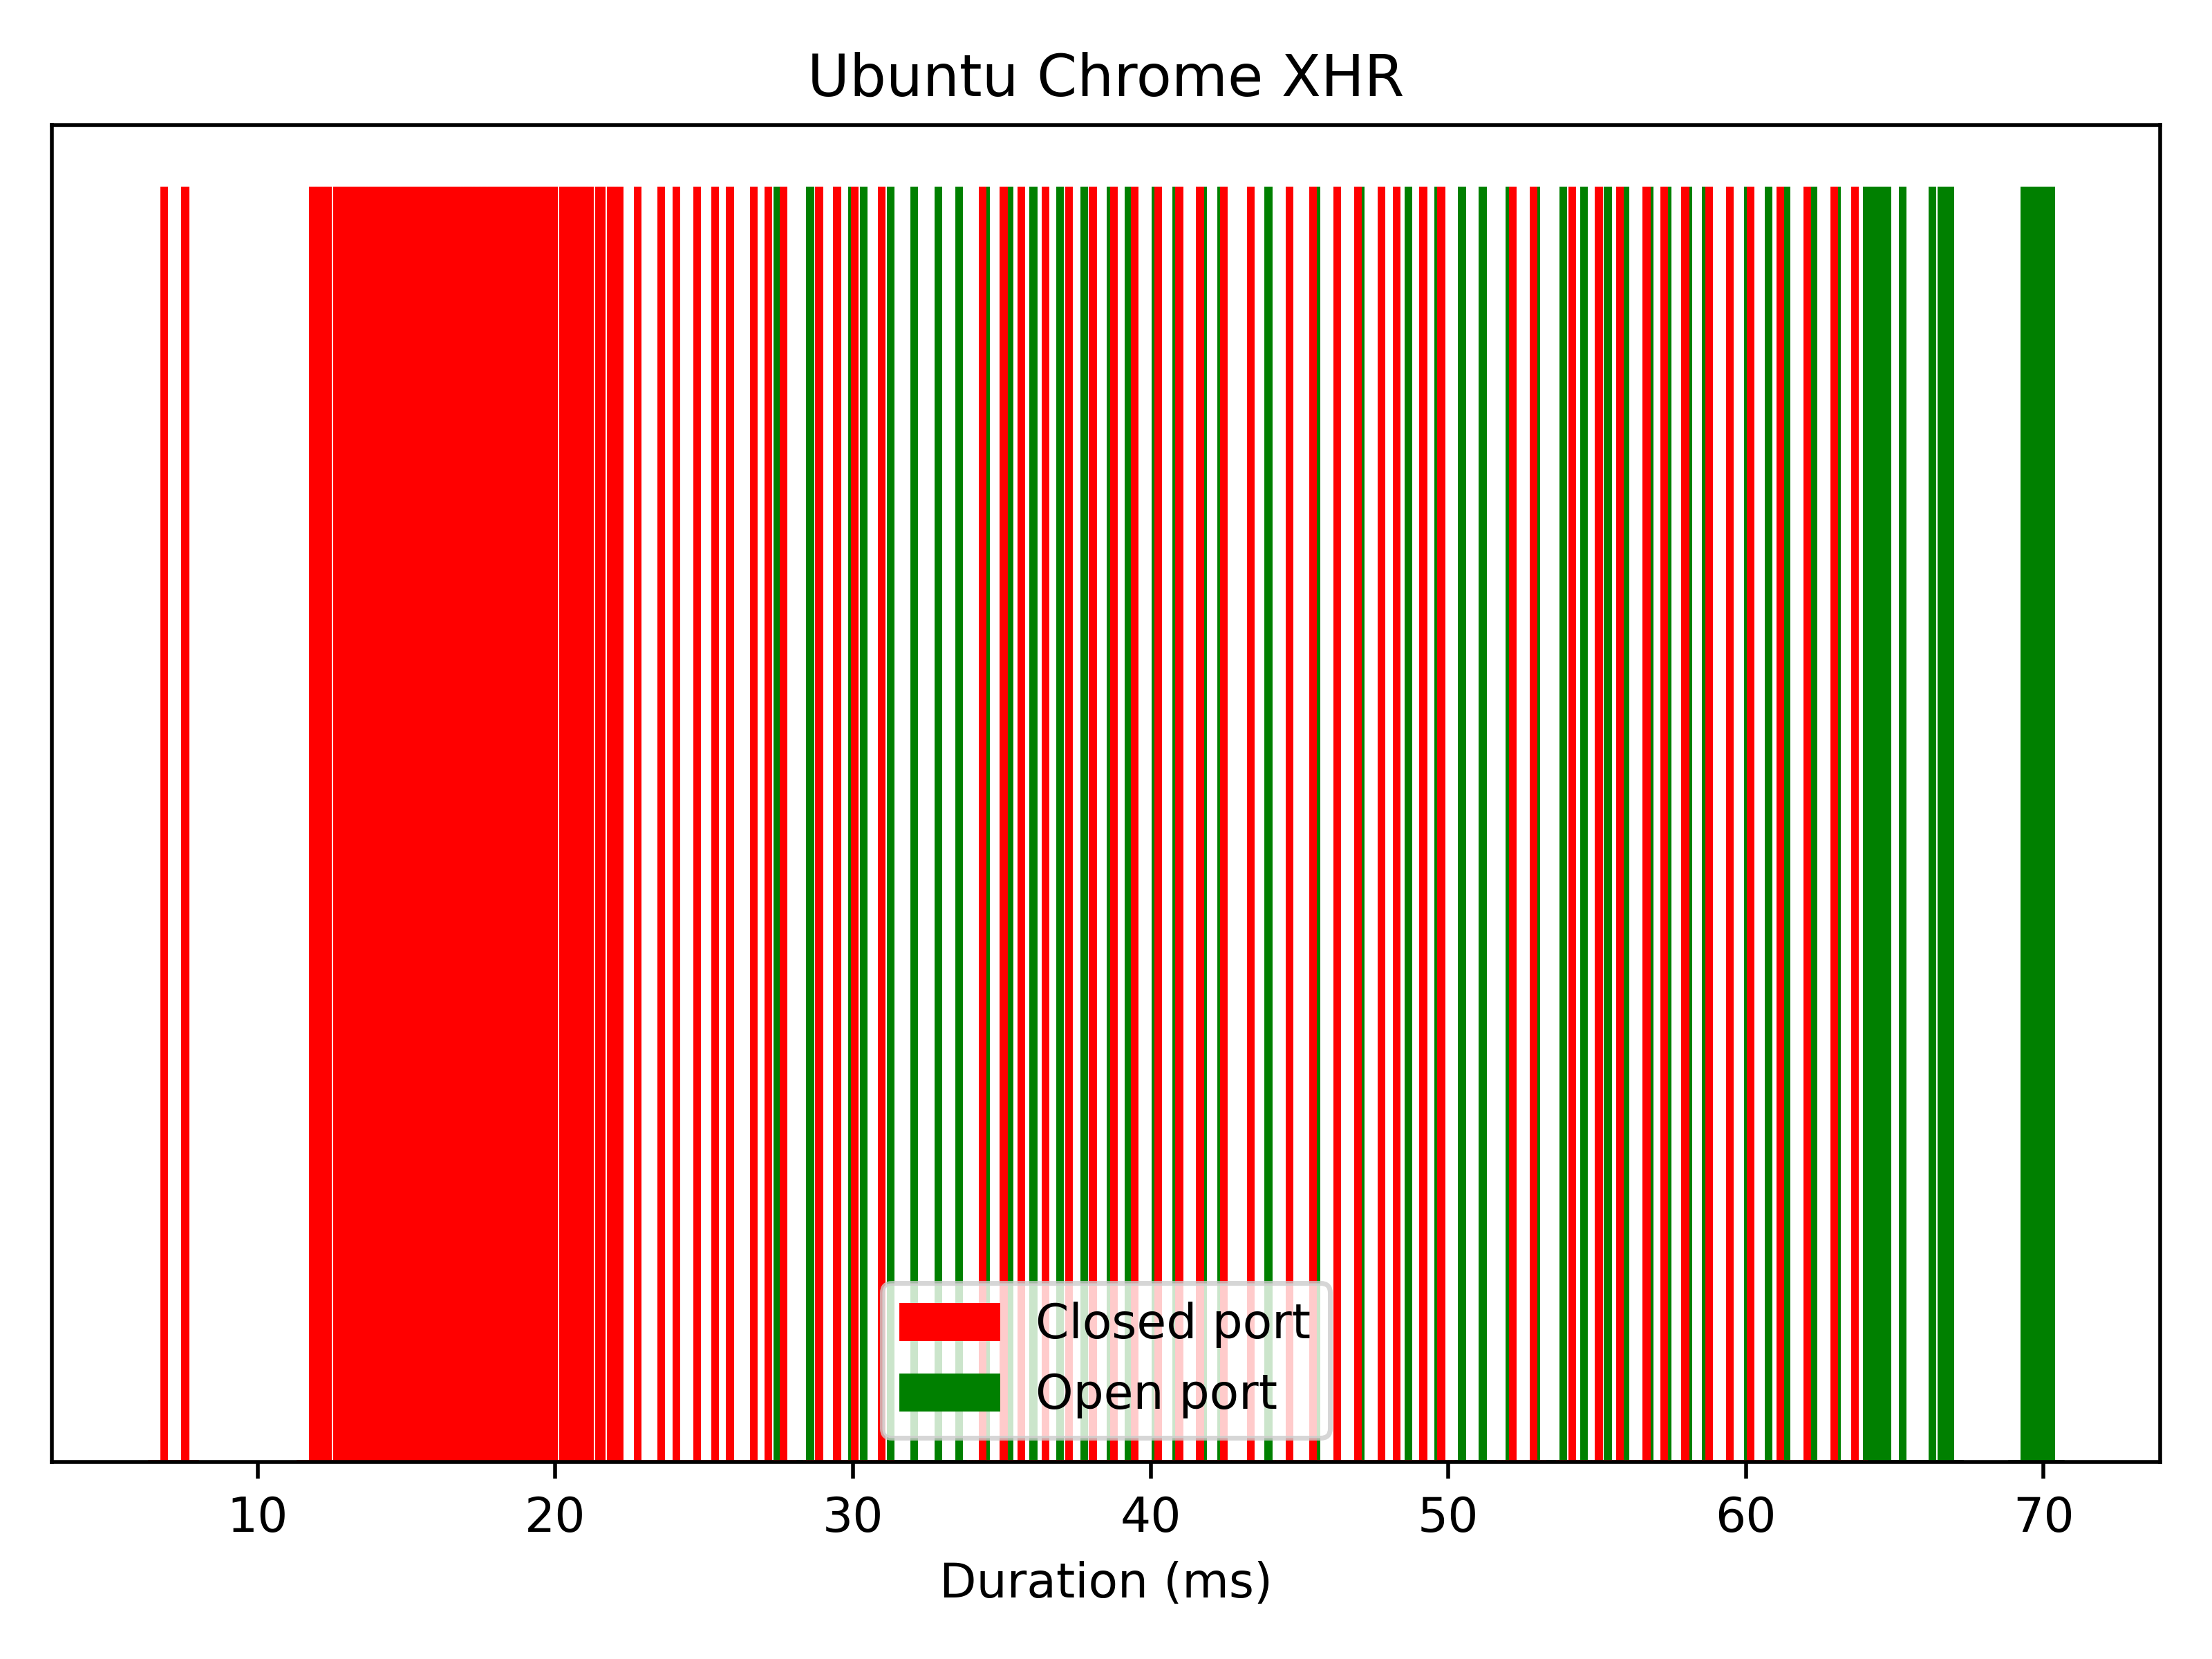
\includegraphics[width=8cm, height=4cm, keepaspectratio]{port_scanning_techniques/img/ubuntu_chrome_efficacy_xhr.png}
    \caption{Ubuntu/Chrome XHR API scan duration open vs closed ports}
    \label{fig:ubuntu-chrome-xhr}
\end{minipage}
\hspace{0.5cm} % Adjust the horizontal space between the two figures
\begin{minipage}{.45\textwidth}
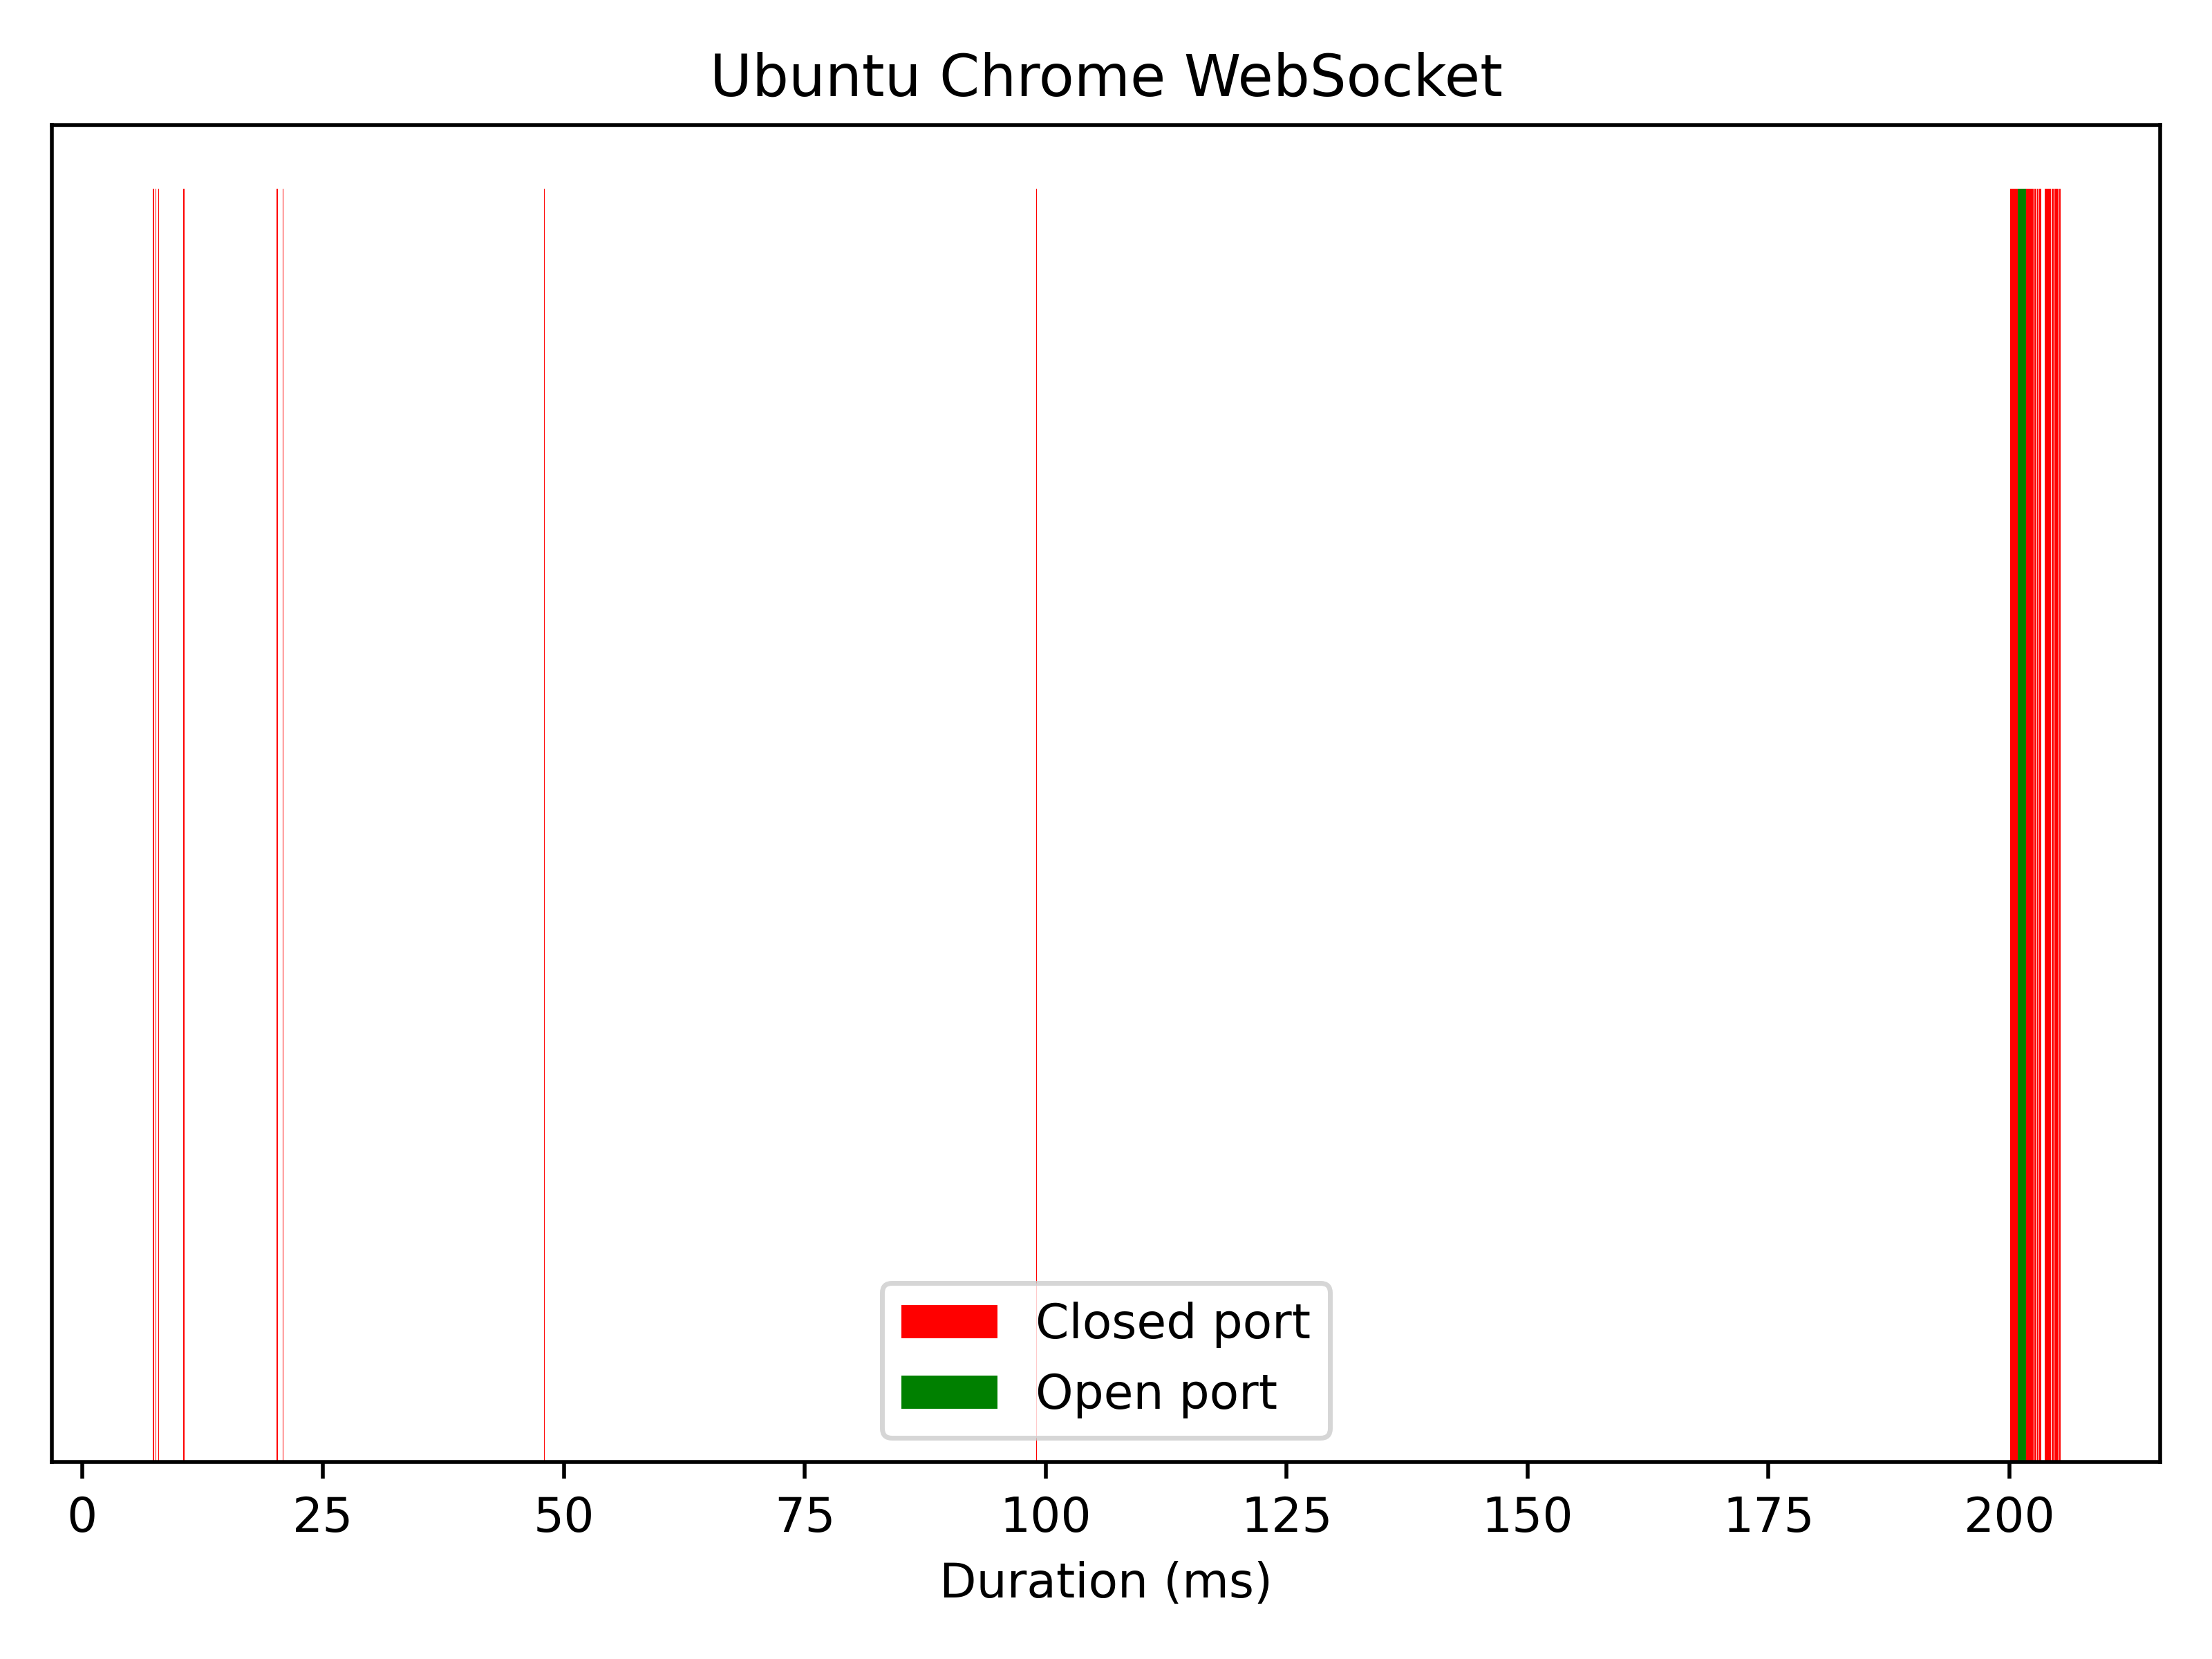
\includegraphics[width=8cm, height=4cm, keepaspectratio]{port_scanning_techniques/img/ubuntu_chrome_efficacy_websocket.png}
    \caption{Ubuntu/Chrome WebSocket API scan duration open vs closed ports}
    \label{fig:ubuntu-chrome-websocket}
\end{minipage}
\end{figure}

\begin{figure}[ht]
\centering
\begin{minipage}{.45\textwidth}
  \centering
\includegraphics[width=8cm, height=4cm, keepaspectratio]{port_scanning_techniques/img/windows_Firefox_efficacy_fetch.png}
    \caption{Windows/Firefox Fetch API scan duration open vs closed ports}
    \label{fig:win-firefox-fetch}
\end{minipage}
\hspace{0.5cm} % Adjust the horizontal space between the two figures
\begin{minipage}{.45\textwidth}
\includegraphics[width=8cm, height=4cm, keepaspectratio]{port_scanning_techniques/img/windows_Firefox_efficacy_xhr.png}
    \caption{Windows/Firefox XHR API scan duration open vs closed ports}
    \label{fig:appendix-win-firefox-xhr}
\end{minipage}
\end{figure}

\begin{figure}[ht]
\centering
\begin{minipage}{.45\textwidth}
  \centering
\includegraphics[width=8cm, height=4cm, keepaspectratio]{port_scanning_techniques/img/windows_Firefox_efficacy_websocket.png}
    \caption{Windows/Firefox WebSocket API scan duration open vs closed ports}
    \label{fig:appendix-win-firefox-websocket}
\end{minipage}
\hspace{0.5cm} % Adjust the horizontal space between the two figures
\begin{minipage}{.45\textwidth}
\includegraphics[width=8cm, height=4cm, keepaspectratio]{port_scanning_techniques/img/ubuntu_Firefox_efficacy_fetch.png}
    \caption{Ubuntu/Firefox Fetch API scan duration open vs closed ports}
    \label{fig:ubuntu-firefox-fetch}
\end{minipage}
\end{figure}

\begin{figure}[ht]
\centering
\begin{minipage}{.45\textwidth}
  \centering
\includegraphics[width=8cm, height=4cm, keepaspectratio]{port_scanning_techniques/img/ubuntu_Firefox_efficacy_xhr.png}
    \caption{Ubuntu/Firefox XHR API scan duration open vs closed ports}
    \label{fig:ubuntu-firefox-xhr}
\end{minipage}
\hspace{0.5cm} % Adjust the horizontal space between the two figures
\begin{minipage}{.45\textwidth}
\includegraphics[width=8cm, height=4cm, keepaspectratio]{port_scanning_techniques/img/ubuntu_Firefox_efficacy_websocket.png}
    \caption{Ubuntu/Firefox WebSocket API scan duration open vs closed ports}
    \label{fig:ubuntu-firefox-websocket}
\end{minipage}
\end{figure}
\clearpage

\section{Scanning techniques efficiency comparison}
\label{appendix:efficiency-comparison}

\begin{figure}[ht]
\begin{adjustwidth}{-3cm}{-1cm}
\centering
\begin{minipage}{.45\textwidth}
  \centering
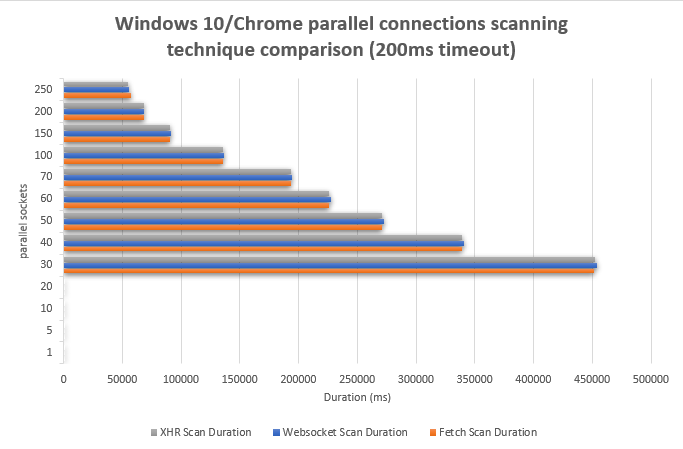
\includegraphics[width=10cm, height=7cm, keepaspectratio]{port_scanning_techniques/img/windows_chrome_scan_technique_comparison.png}
    \caption{Windows/Chrome Parallel sockets efficiency comparison}
    \label{fig:appendix-windows_chrome_n_sockets}
\end{minipage}
\hspace{3cm} % Adjust the horizontal space between the two figures
\begin{minipage}{.45\textwidth}
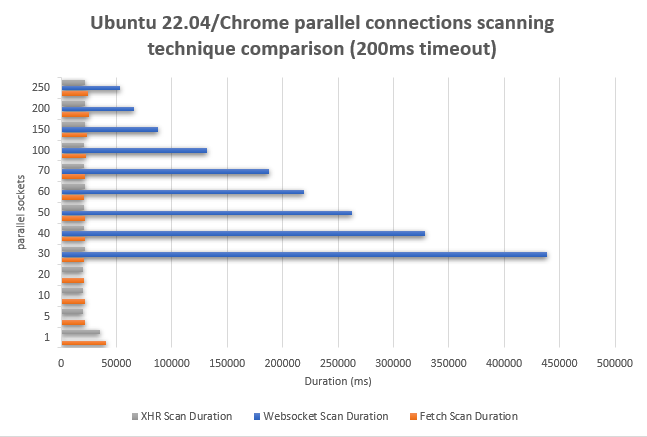
\includegraphics[width=10cm, height=7cm, keepaspectratio]{port_scanning_techniques/img/ubuntu_chrome_scan_technique_comparison.png}
    \caption{Ubuntu/Chrome Parallel sockets efficiency comparison}
    \label{fig:appendix-ubuntu_chrome_n_sockets}
\end{minipage}
\end{adjustwidth}
\end{figure}

\begin{figure}[ht]
\begin{adjustwidth}{-3cm}{-1cm}
\centering
\begin{minipage}{.45\textwidth}
  \centering
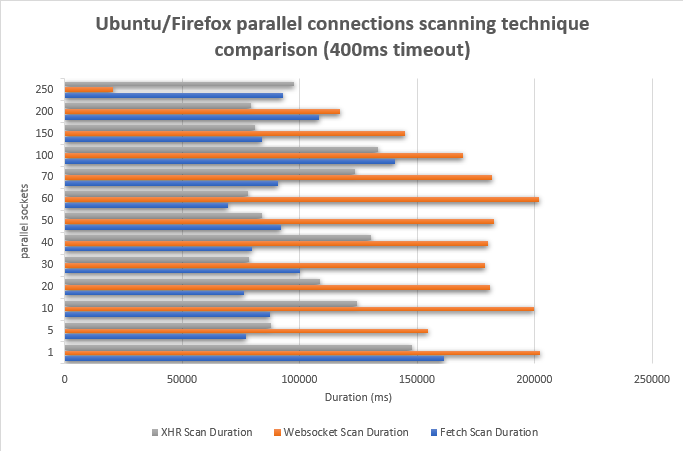
\includegraphics[width=10cm, height=7cm, keepaspectratio]{port_scanning_techniques/img/ubuntu_firefox_scan_technique_comparison.png}
    \caption{Ubuntu/Firefox Parallel sockets efficiency comparison}
    \label{fig:ubuntu_firefox_n_sockets}
\end{minipage}
\hspace{3cm} % Adjust the horizontal space between the two figures
\begin{minipage}{.45\textwidth}
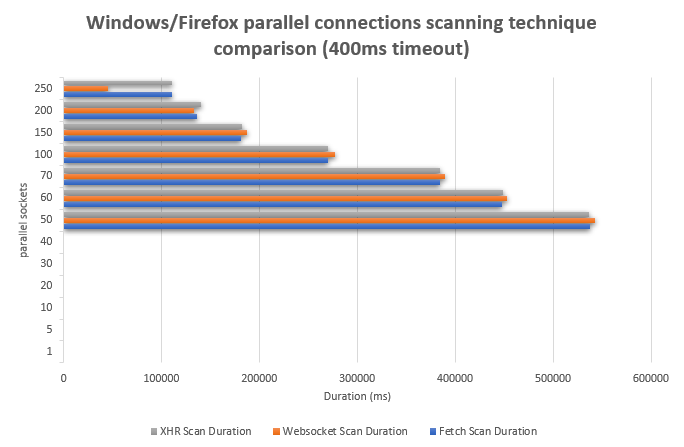
\includegraphics[width=10cm, height=7cm, keepaspectratio]{port_scanning_techniques/img/windows_firefox_scan_technique_comparison.png}
    \caption{Windows/Firefox Parallel sockets efficiency comparison}
    \label{fig:windows_firefox_n_sockets}
\end{minipage}
\end{adjustwidth}
\end{figure}